% ═══════════════════════════════════════════════════════════════════════════
%  Part 5 - PCB Design & KiCad Workflow
% ═══════════════════════════════════════════════════════════════════════════

\section{PCB Design \& KiCad Workflow}

This section documents the complete PCB design process - from tool selection
and library creation through schematic entry, layout, and DRC resolution.
The workflow reflects our realities as first-time KiCad users inheriting an
incomplete project from a teammate.

% ─── Design Tool Selection ────────────────────────────────────────────────
\subsection{Design Tool Selection}

KiCad~9.0 was chosen as the EDA tool for the following reasons:

\begin{itemize}[leftmargin=1.8em, itemsep=2pt]
  \item \textbf{Free and open-source} - no licence cost or seat restrictions
  \item \textbf{University standard} - recommended by the department for
        coursework submissions
  \item \textbf{Full-featured} - schematic capture, PCB layout, 3D viewer,
        Gerber export, and DRC in a single package
\end{itemize}


% ─── Custom Symbol & Footprint Creation ──────────────────────────────────
\subsection{Custom Symbol \& Footprint Creation}

Several components on the Phase~3 board have no standard KiCad library parts.
Custom symbols and/or footprints were created for each:

\begin{itemize}[leftmargin=1.8em, itemsep=2pt]
  \item \chip{RDA5807M} module - 11$\times$11\,mm, 2$\times$5 pads,
        1.27\,mm pitch (castellation footprint, no standard library match)
  \item \chip{PAM8403} (SOP-16) - custom symbol with correct pin mapping
  \item \chip{TP4056} (SOP-8) - custom symbol
  \item \chip{CH340C} (SOP-16) - custom symbol
  \item \chip{HT7333} (SOT-89) - custom symbol
  \item \chip{FS8205A} (SOT-23-6) - custom symbol
\end{itemize}

\begin{logentry}{4}{Feb 17 \textbullet{} Custom RDA5807M symbol}
First attempt at creating a custom KiCad symbol for the \chip{RDA5807M} module.
Made critical errors: used wrong pin types (all set to \texttt{Passive} instead
of \texttt{Bidirectional} for SDA/SCL, \texttt{Power I/O} for VCC/GND,
\texttt{Output} for LOUT/ROUT).  Also had no pin numbers - only names.  KiCad
couldn't match symbol pins to footprint pads.  Required complete rebuild of the
symbol.
\end{logentry}

% ─── Library Path Issues ─────────────────────────────────────────────────
\subsection{Library Path Issues}

\begin{calloutwarn}[Library Path Hell]
The KiCad project referenced the teammate's old PC paths
(\texttt{C:\textbackslash Users\textbackslash OtherUser\textbackslash\ldots})
in \texttt{fp-lib-table} and \texttt{sym-lib-table}.  Every footprint showed
\emph{``not found''}.  Fix: replace all absolute paths with
\texttt{\$\{KIPRJMOD\}} variable for portability.  Also discovered the
\chip{TP4056} entry was pointing to the \chip{PAM8403} folder due to a
copy-paste error.
\end{calloutwarn}

% ─── Schematic Entry ─────────────────────────────────────────────────────
\subsection{Schematic Entry}

After resolving library paths and rebuilding custom symbols, the schematic was
entered and validated using KiCad's Electrical Rules Check (ERC).

\subsubsection{ERC Results}

\begin{itemize}[leftmargin=1.8em, itemsep=2pt]
  \item \textbf{Initial run:} 1~error + 18~warnings
  \item \textbf{Fixed:} \texttt{power\_pin\_not\_driven} error - a power flag
        was missing on the battery net
  \item \textbf{Remaining warnings:} bidirectional pin conflicts
        (\chip{PAM8403} symbol pin types), unconnected pins (acceptable -
        unused MCU I/O)
  \item \textbf{Final ERC:} 0~errors, 4~warnings (SW1/SW2 mechanical pads -
        ignorable)
\end{itemize}

% ─── PCB Layout ──────────────────────────────────────────────────────────
\subsection{PCB Layout}

\subsubsection{Board Outline \& Mechanical}

\begin{itemize}[leftmargin=1.8em, itemsep=2pt]
  \item Board dimensions: 70\,$\times$\,50\,mm rectangle
  \item Corner treatment: 2\,mm fillet (rounded corners)
  \item Mounting: M3 holes at all four corners
\end{itemize}

\subsubsection{Design Rules}

\begin{itemize}[leftmargin=1.8em, itemsep=2pt]
  \item Minimum trace width: 0.25\,mm (signal traces)
  \item Power traces: 0.5–1.0\,mm (VBAT, +3V3 distribution)
  \item Clearance: 0.2\,mm minimum copper-to-copper
  \item Via drill: 0.3\,mm
\end{itemize}

\subsubsection{Layer Stackup}

\begin{itemize}[leftmargin=1.8em, itemsep=2pt]
  \item \textbf{Top (F.Cu):} all components + signal traces
  \item \textbf{Bottom (B.Cu):} continuous GND copper pour (ground plane)
\end{itemize}

\subsubsection{Zone Separation}

The board is divided into functional zones to minimise interference:

\begin{itemize}[leftmargin=1.8em, itemsep=2pt]
  \item \textbf{Analog (west side):} \chip{RDA5807M}, audio mixing network,
        headphone jack
  \item \textbf{Digital (east side):} \chip{ATmega328P}, \chip{SSD1306} OLED,
        encoders
  \item \textbf{Power (south-west):} \chip{TP4056}, \chip{DW01A}/\chip{FS8205A},
        \chip{HT7333}, battery connector
\end{itemize}

\subsubsection{Component Placement Rationale}

\begin{itemize}[leftmargin=1.8em, itemsep=2pt]
  \item USB-C connector at bottom edge (accessible for cable insertion)
  \item OLED display at top (visible when radio is held)
  \item Rotary encoders at left and right sides (ergonomic thumb access)
  \item \chip{RDA5807M} placed away from \chip{PAM8403} (minimise Class-D
        switching noise coupling into RF front-end)
\end{itemize}

% ─── Autorouter Attempt ──────────────────────────────────────────────────
\subsection{Autorouter Attempt}

\begin{calloutfail}[Autorouter Failure]
First attempt used the Freerouting autorouter.  Result: 137~DRC violations
including shorts, no-net vias, and clearance violations.  The autorouter
created ghost traces and unconnected copper fragments.  All autorouted traces
were deleted and manual routing was performed instead.
\end{calloutfail}


% ─── Lessons from PCB Design ─────────────────────────────────────────────
\subsection{Lessons from PCB Design}

\begin{description}[style=nextline, leftmargin=1.5em, itemsep=4pt,
                    font=\sffamily\bfseries\color{brandteal}]
  \item[\texttt{\$\{KIPRJMOD\}} saves portability headaches]
    Always use project-relative paths in \texttt{fp-lib-table} and
    \texttt{sym-lib-table}.  Absolute paths break the moment the project moves
    to another machine.

  \item[Custom symbols need correct pin types from the start]
    Setting all pins to \texttt{Passive} silences ERC but hides real wiring
    errors.  Use \texttt{Power I/O}, \texttt{Bidirectional}, \texttt{Output},
    etc.\ as appropriate.

  \item[Autorouters fail on mixed-signal boards]
    Manual routing is required for boards combining RF, analog audio, and
    digital logic.  The autorouter cannot understand zone separation or
    sensitive signal isolation.

  \item[DRC markers can be hidden during routing]
    Appearance Panel $\to$ Objects $\to$ ``DRC Markers'' $\to$ click the eye
    icon.  Markers still exist in the DRC list but won't clutter the canvas.

  \item[One ghost trace can generate dozens of DRC arrows]
    A single leftover copper fragment from incomplete routing creates a chain
    reaction of violations (shorts, clearance, unconnected nets).  Always
    inspect and delete orphan traces.

  \item[Crystal must be within 10\,mm of MCU oscillator pins]
    Long traces to the crystal add parasitic capacitance and can prevent
    oscillator startup.  Keep Y1 as close to \pin{XTAL1}/\pin{XTAL2} as
    physically possible.

  \item[Ground plane continuity requires stitching vias]
    Where components on the top layer block the bottom copper pour, add
    stitching vias on both sides of the gap to maintain a low-impedance
    return path.
\end{description}

% ─── Schematic & PCB Images ────────────────────────────────────────────────
\subsection{Schematic \& PCB Images}

\begin{figure}[H]
\centering
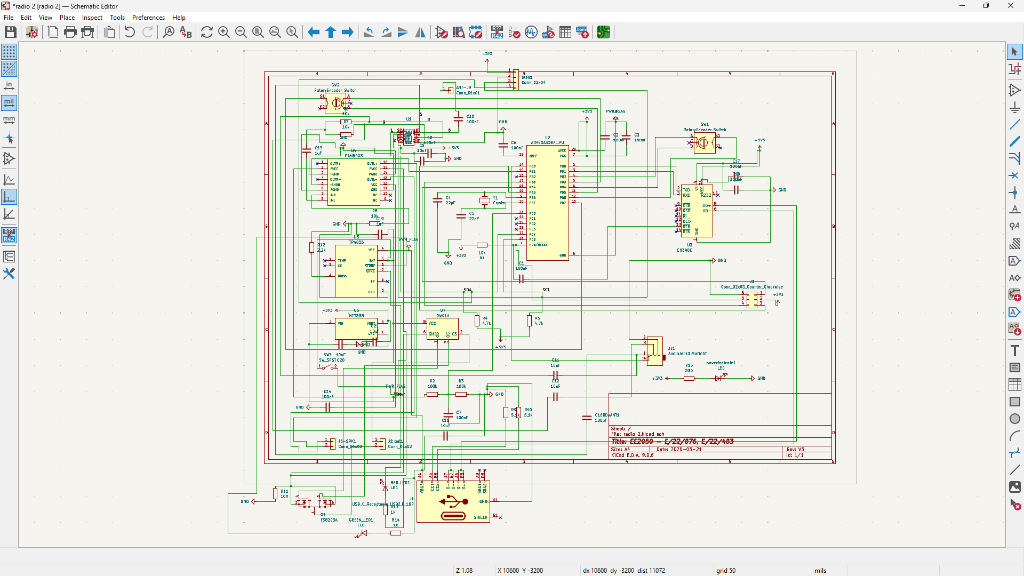
\includegraphics[width=0.9\linewidth]{images/schematic.png}
\caption{Phase~3 KiCad Schematic.}
\label{fig:kicad-schematic}
\end{figure}

\begin{figure}[H]
\centering
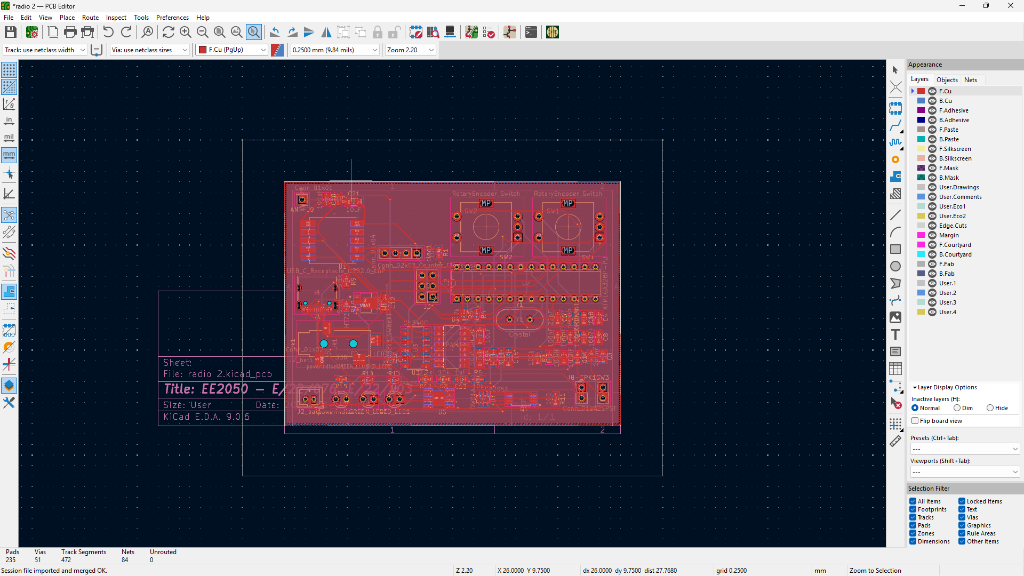
\includegraphics[width=0.9\linewidth]{images/radio2_top.png}
\caption{Phase~3 PCB layout (KiCad PCB Editor) showing fully routed traces.}
\label{fig:pcb-top}
\end{figure}

\begin{figure}[H]
\centering
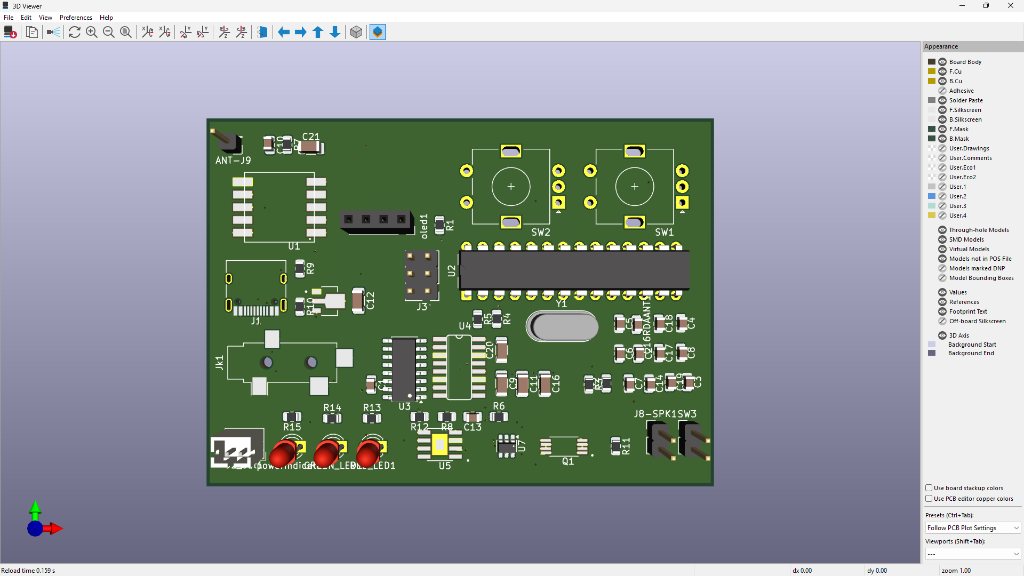
\includegraphics[width=0.9\linewidth]{images/RADIO.png}
\caption{3D render of the PCB (custom component models omitted).}
\label{fig:pcb-3d}
\end{figure}
